%Thema und Aufgabenstellung
 
%\pagestyle{scrheadings}

\chapter*{Thema und Aufgabenstellung}
\markboth{Thema und Aufgabenstellung}{Thema und Aufgabenstellung}
\textbf{Thema:}\par\smallskip
 
Erstellung einer \LaTeX-Vorlage für Abschlussarbeiten
\par\smallskip  
WICHTIG bitte nur die Hauptdatei kompilieren nicht die ausgelagerten externen Dateien sonst kommt es zu Fehlermeldungen!\par
Als Editor ist TexStudio oder TexMaker geeignet!\\

\begin{figure}[h!]
  \begin{centering}
  {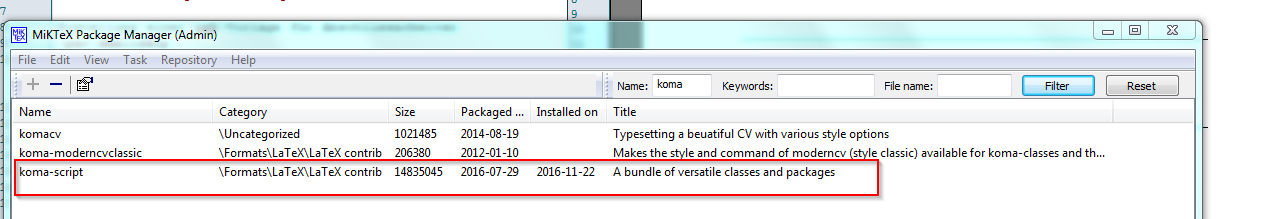
\includegraphics[scale=0.5]{Abbildungen/koma_script_update.png}
   \caption{Bitte ein update der KomaSkript-Klasse machen}}
  \end{centering}
  \end{figure}
  

\begin{figure}[h!]
  \begin{centering}
  {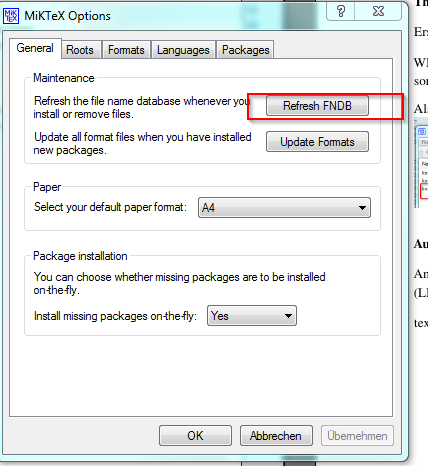
\includegraphics[scale=0.5]{Abbildungen/refresh_fndb.png}\hfill
\caption{und unter MiteX 2.9 einen Refresh ausführen}}
  \end{centering}
  \end{figure}




\par\bigskip
\textbf{Aufgabenstellung:}\par\smallskip
Am Lehrstuhl für Informationstechnik mit dem Schwerpunkt Kommuniktaionselektronik (LIKE)
\par\smallskip  
Text der Aufgabenstellung hier ...


